
\subsection{Hierarchy}


\begin{frame}[c]{Why Hierarchy?}
    \Large
    \pause
    If there is a connection cost, hierarchies are more efficient \cite{mengistu2016evolutionary}. 
    
    \pause
    Especially when tasks change regularly.
\end{frame}


\begin{frame}[c]{Why Hierarchy? II}
    \Large
    \begin{itemize}[<+(1)->]
        \item Reduced Training Time
        \item Reduced Memory Usage
        \item Introduce Generalizations
        \item Learned patterns are recombined at higher levels
        \item Transfer Learning
    \end{itemize}
\end{frame}


\begin{frame}[c]{What Hierarchy}
    \pause
                                        % trim = left bottom right top
    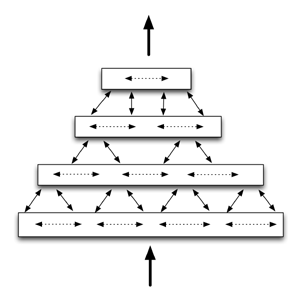
\includegraphics[width=\textwidth, trim = 0 55 0 60, clip]{hierarchy}
\end{frame}


\begin{frame}[c]{Example Application}
    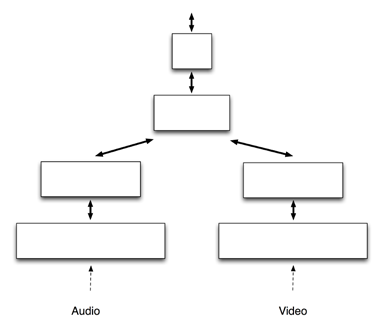
\includegraphics[height=0.9\textheight]{hierarchy_2} 
\end{frame}


\begin{frame}[c]{How Many Levels?}
    \Large
    \begin{itemize}[<+(1)->]
        \item They always learn the best representation
        \item Tradeoff between depth and layer size
        \item Simple problems can be solved with one region
    \end{itemize}
\end{frame}



\subsection{Regions}


\begin{frame}[c]{Region - Introduction}
    \pause
                                        % trim = left bottom right top
    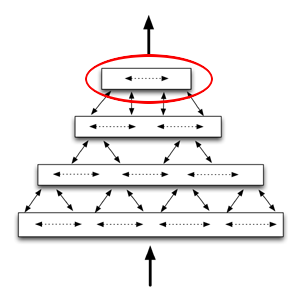
\includegraphics[width=\textwidth, trim = 0 55 0 54, clip]{region}
\end{frame}


\begin{frame}[c]{Region - Details}
    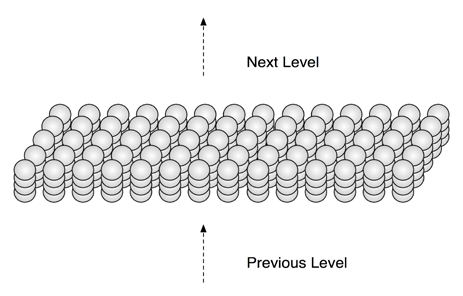
\includegraphics[width=\textwidth]{region_2}
\end{frame}


\begin{frame}[c]{Region - Attributes}
    \begin{itemize}[<+(1)->]
        \item All Regions do basically the same
        \item Based on Biological Regions in the Brain
        \item HTM Regions are similar to Layer 3 of the Neocortex
        \item Can do Inference and Prediction even on complex data
    \end{itemize}
\end{frame}


